\documentclass{beamer}
\usepackage{appendixnumberbeamer}

\mode<presentation>{\usetheme[subsectionpage=progressbar,block=fill,numbering=none]{metropolis}}

\usepackage[sfdefault]{FiraSans} %% option 'sfdefault' activates Fira Sans as the default text font
\usepackage[english]{babel}
% \usepackage[utf8]{inputenc}

\usepackage{graphicx} % Allows including images
\usepackage{caption}
\usepackage{booktabs} % Allows the use of \toprule, \midrule and \bottomrule in tables
\usepackage{multicol}

% Math packages
\usepackage{amsmath}
\usepackage{mathtools}
\usepackage{amssymb}
\usepackage{mathpartir}
\usepackage{stmaryrd}
\usepackage{centernot}
\usepackage[normalem]{ulem}

%% Coding
\usepackage[outputdir=build]{minted}

% Coloured boxes
\usepackage{tcolorbox}
\colorlet{alert}{mLightBrown}
\colorlet{mLightBrownTransparent}{white!70!mLightBrown}
\newtcolorbox{alertbox}
{standard jigsaw, opacityback=0,colframe=alert}
\newtcolorbox{tbox}
{standard jigsaw, opacityback=0,opacityframe=0}

%% Quotes with author
\usepackage{xparse}

\let\oldquote\quote
\let\endoldquote\endquote

\RenewDocumentEnvironment{quote}{o}
  {\oldquote}
  {\IfValueT{#1}{\par\nobreak
   \hfill--- #1}\endoldquote\addvspace{\smallskipamount}}

\newcommand{\dotcup}{\mathbin{\mathaccent\cdot\cup}}
\newcommand{\fromto}[2]{\{#1,\dotsc,#2\}}
\newcommand{\denot}[1]{\llbracket#1\rrbracket}
\newcommand{\listt}[1]{\mathsf{List}~#1}
\newcommand{\map}{\mathsf{map}}
\newcommand{\haskell}[1]{\mintinline{haskell}{#1}}
\newcommand{\vint}[1]{\mathcal{V}\denot{#1}}
\newcommand{\tint}[1]{\mathcal{E}\denot{#1}}
\newcommand{\wt}[1]{\mathsf{wt}_{#1}}
\newcommand{\rels}{\mathcal{R}}
\newcommand{\values}{Val}
\newcommand{\bool}{\mathsf{Bool}}
\newcommand{\nat}{\mathsf{Nat}}
\newcommand{\zero}{\mathsf{0}}
\newcommand{\suc}{\mathsf{succ}}
\newcommand{\pair}{\mathsf{pair}}
\newcommand{\true}{\mathsf{true}}
\newcommand{\false}{\mathsf{false}}
\newcommand{\nil}{\mathsf{nil}}
\newcommand{\cons}{\mathsf{cons}}
\newcommand{\length}{\mathsf{length}}
\newcommand{\eq}{\mathsf{eq}}
\newcommand{\cmp}{\mathsf{cmp}}
\newcommand{\nf}[1]{#1{\downarrow}}
\newcommand{\eqnf}{=^*}


\title{Theorems for Free!} % the title on the title page
\subtitle{by Philip Wadler}

\author{Kevin Kappelmann} % Your name
\institute[TU Munich]{Technical University of Munich}
\date{May 27, 2021} % Date, can be changed to a custom date

\begin{document}

\maketitle

%------------------------------------------------
\section{Type Systems and Polymorphism}
% \begin{frame}[fragile]{Haskell Has Types}

% \begin{minted}{haskell}
% appTwice :: (Int -> Int) -> Int -> Int
% appTwice f x = f (f x)
% \end{minted}

% \pause
% \centering What is the result of\dotso

% \begin{uncoverenv}<3>
% \begin{onlyenv}<1-3>
% \begin{minted}{haskell}
% appTwice (*2) 1 = ?
% \end{minted}
% \end{onlyenv}
% \end{uncoverenv}

% \begin{onlyenv}<4>
% \begin{minted}{haskell}
% appTwice (*2) 1 = 4
% \end{minted}
% \end{onlyenv}

% \begin{onlyenv}<5>
% \begin{minted}{haskell}
% appTwice (*2) 1 = 4
% appTwice (*2) "bogus" = ?
% \end{minted}
% \end{onlyenv}

% \begin{onlyenv}<6>
% \begin{minted}{haskell}
% appTwice (*2) 1 = 4
% appTwice (*2) "bogus" = ...
% \end{minted}
% \begin{alertbox}
% \begin{minted}[escapeinside=??]{bash}
% • Couldn?'?t match expected type ‘Int’ with
  % actual type ‘[Char]’
% • In the second argument of ‘appTwice’,
  % namely ‘"bogus"’
  % In the expression: appTwice (*2) "bogus"...
% \end{minted}
% \end{alertbox}
% \end{onlyenv}
% \end{frame}

% \begin{frame}
% \centering
% \Huge Thank you, type system!
% \end{frame}

% \begin{frame}{What is a Type System?}

% {\Large Type systems are mechanisms that guarantee the absence of certain programming errors.}

% \pause
% \vspace{3\baselineskip}
% \centering{\alert{\large \dotso is there a catch?}}
% \end{frame}

\begin{frame}[fragile]{Sigh, Just Apply It Twice!}
\begin{minted}{haskell}
appTwice :: (Int -> Int) -> Int -> Int
appTwice f x = f (f x)
\end{minted}

\centering What is the result of\dotso

\begin{onlyenv}<1-2>
\begin{uncoverenv}<2>
\begin{minted}{haskell}
appTwice (*2) 1 = ?
\end{minted}
\end{uncoverenv}
\end{onlyenv}

\begin{onlyenv}<3>
\begin{minted}{haskell}
appTwice (*2) 1 = 4
\end{minted}
\end{onlyenv}

\begin{onlyenv}<4>
\begin{minted}{haskell}
appTwice (*2) 1 = 2
appTwice (*2) "bogus" = ?
\end{minted}
\end{onlyenv}

\begin{onlyenv}<5>
\begin{minted}{haskell}
appTwice (*2) 1 = 2
appTwice (*2) "bogus" = ...
\end{minted}
\end{onlyenv}

\begin{onlyenv}<1-5>
\begin{uncoverenv}<5>
\begin{alertbox}
\begin{minted}[escapeinside=??]{bash}
• Couldn?'?t match expected type ‘Int’ with
  actual type ‘[Char]’
• In the second argument of ‘appTwice’,
  namely ‘"bogus"’
  In the expression: appTwice (*2) "bogus"...
\end{minted}
\end{alertbox}
\end{uncoverenv}
\end{onlyenv}

\begin{onlyenv}<6>
\begin{minted}{haskell}
appTwice (*2) 1 = 2
appTwice (++"l") "haske" = ?
\end{minted}
\end{onlyenv}

\begin{onlyenv}<7>
\begin{minted}{haskell}
appTwice (*2) 1 = 2
appTwice (++"l") "haske" = ...
\end{minted}
\end{onlyenv}

\begin{onlyenv}<6->
\begin{uncoverenv}<7->
\begin{alertbox}
\begin{minted}[escapeinside=??]{bash}
• Couldn?'?t match type ‘[Char]’ with ‘Int’
  Expected type: Int -> Int
  Actual type: [Char] -> [Char]
• In the first argument of ‘appTwice’,
  namely ‘(++"l")’
  In the expression: appTwice (++"l") "haske"...
\end{minted}
\end{alertbox}
\end{uncoverenv}
\end{onlyenv}

\end{frame}

% \begin{frame}[fragile]{Do Not Repeat Yourself}
% Well then, let us fix this problem:

% \begin{onlyenv}<1-3>
% \begin{uncoverenv}<2-3>
% \begin{minted}{haskell}
% appTwiceInt :: (Int -> Int) -> Int -> Int}
% appTwiceInt f x = f (f x)

% appTwiceString :: (String -> String) -> String -> String
% appTwiceString f x = f (f x)
% \end{minted}
% \end{uncoverenv}
% \end{onlyenv}

% \begin{onlyenv}<4>
% \begin{minted}[highlightlines={2,5},highlightcolor=mLightBrownTransparent]{haskell}
% appTwiceInt :: (Int -> Int) -> Int -> Int}
% appTwiceInt f x = f (f x)

% appTwiceString :: (String -> String) -> String -> String
% appTwiceString f x = f (f x)
% \end{minted}
% \end{onlyenv}
% \only<1-3>{\uncover<3>{And we are happy again:}}
% \only<4>{And we are \sout{happy} \alert{unhappy} again:}

% \begin{uncoverenv}<3->
% \begin{minted}{haskell}
% appTwiceInt (*2) 1 = 4
% appTwiceSting (++"l") "haske" = "haskell"
% \end{minted}
% \end{uncoverenv}
% \end{frame}

% \begin{frame}{The \emph{Abstraction Principle}}
% \begin{quote}[Benjamin Pierce]
% Each significant piece of functionality in a program should be implemented in just one place in the source code. Where similar functions are carried out by distinct pieces of code, it is generally beneficial to combine them into one by abstracting out the varying parts.
% \end{quote}
% \end{frame}

\begin{frame}[fragile]{Polymorphism to the Rescue!}
Haskell knows \emph{parametric polymorphism}: we
can abstract over types by using type variables.

\pause

\begin{minted}{haskell}
appTwice :: (a -> a) -> a -> a
appTwice f x = f (f x)
\end{minted}

\pause
And we are happy:

\begin{minted}{haskell}
appTwice (*2) 1 = 4
appTwice (++"l") "haske" = "haskell"
\end{minted}

\pause
\centering {\large End of the story? \pause \alert{Of course not!}}

\end{frame}

\begin{frame}
\centering {\Huge Polymorphism comes with another twist!}
\end{frame}

\begin{frame}[fragile]{Black Magic}
I show you a term's type but not its definition.
You tell me the possible results:
\footnote{Let us forget about \mintinline{haskell}{undefined} for a moment.}

% \begin{uncoverenv}<2>
% \begin{onlyenv}<1-2>
% \begin{minted}{haskell}
% f :: a -> b -> a
% -- def. of f hidden

% f 42 "hi" = ?
% f "hi" 42 = ?
% \end{minted}
% \end{onlyenv}
% \end{uncoverenv}

% \begin{onlyenv}<3>
% \begin{minted}{haskell}
% f :: a -> b -> a
% -- def. of f hidden

% f 42 "hi" = 42
% f "hi" 42 = "hi"
% \end{minted}
% \end{onlyenv}

% \begin{onlyenv}<4>
% \begin{minted}{haskell}
% f :: a -> b -> a
% f x y = x

% f 42 "hi" = 42
% f "hi" 42 = "hi"
% \end{minted}
% \end{onlyenv}

\begin{uncoverenv}<2>
\begin{onlyenv}<1-2>
\begin{minted}{haskell}
g :: (a -> a) -> a -> a
-- def. of g hidden

g (*2) 1 =? 1
g (*2) 1 =? 2
g (*2) 1 =? 3
g (*2) 1 =? 16
g (*2) 1 =? 42
\end{minted}
\end{onlyenv}
\end{uncoverenv}

\begin{onlyenv}<3-4>
\begin{minted}[highlightlines={4,5,7},highlightcolor=mLightBrownTransparent]{haskell}
g :: (a -> a) -> a -> a
-- def. of g hidden

g (*2) 1 =? 1
g (*2) 1 =? 2
g (*2) 1 /= 3
g (*2) 1 =? 16
g (*2) 1 /= 42
\end{minted}
\end{onlyenv}

\begin{onlyenv}<5>
\begin{minted}[highlightlines={7},highlightcolor=mLightBrownTransparent]{haskell}
g :: (a -> a) -> a -> a
-- def. of g hidden

g (*2) 1 /= 1
g (*2) 1 /= 2
g (*2) 1 /= 3
g (*2) 1 = 16
g (*2) 1 /= 42
\end{minted}
\end{onlyenv}

\begin{onlyenv}<6>
\begin{minted}[highlightlines={7},highlightcolor=mLightBrownTransparent]{haskell}
g :: (a -> a) -> a -> a
g f x = f (f (f (f x)))

g (*2) 1 /= 1
g (*2) 1 /= 2
g (*2) 1 /= 3
g (*2) 1 = 16
g (*2) 1 /= 42
\end{minted}
\end{onlyenv}


\uncover<4-6>{
What if I told you that \mintinline{haskell}{g (++"I") "" = "IIII"}?
}
\end{frame}

\begin{frame}
\Large Polymorphic functions are defined once and for all for any type and as such must work uniformly on values of any type.

\pause

\Large From the type of a polymorphic function,
we can derive a theorem that it satisfies.
\end{frame}

\begin{frame}
\centering \huge Polymorphic types provide us \emph{theorems for free}.
\end{frame}

\section{Technical Development}

\begin{frame}{System F}

The polymorphic lambda calculus aka System F:

\pause
Types:
\begin{equation*}
\tau \Coloneqq  \alpha \mid \tau \to \tau \mid \forall \alpha.\ \tau
\end{equation*}

\pause
Terms:
\begin{equation*}
t \Coloneqq x \mid \lambda x : \tau.\ t \mid t\, t \mid \Lambda \alpha.\ t \mid  t\,[\tau]
\end{equation*}

\pause
Values:
\begin{equation*}
v \Coloneqq x\mid \lambda x : \tau.\ t \mid \Lambda \alpha.\ t
\end{equation*}


\pause
Here is our \mintinline{haskell}{appTwice} function:
\begin{align*}
&\Lambda \alpha.\,\lambda f : \alpha\to\alpha.\,\lambda x : \alpha.\, f\ (f\, x) : \forall \alpha.\, (\alpha\to\alpha)\to\alpha\to\alpha
\end{align*}

\pause

We can call it like this: \mintinline{haskell}{appTwice [Int] (+1) 0}
\end{frame}

\begin{frame}[fragile]{Types as Relations}
\only<1>{It is natural to interpret a type $\tau$ as a set $\denot{\tau}$ containing all values of type $\tau$, e.g. $\denot{\mintinline{haskell}{Bool}}=\{\mintinline{haskell}{True,False}\}$ in Haskell.}
\only<2>{\sout{It is natural to interpret a type $\tau$ as a set $\denot{\tau}$ containing all values of type $\tau$, e.g. $\denot{\mintinline{haskell}{Bool}}=\{\mintinline{haskell}{True,False}\}$ in Haskell.}}

% \pause

% The key idea to derive free theorems is to instead interpret a \emph{type as a relation} that
% \begin{enumerate}[<+->]
% \item relates terms of the given type and
% \item whose membership is preserved under eliminating forms.
% \end{enumerate}

\vspace{\baselineskip}

\uncover<2>{\centering \Large New slogan: \alert{types relate terms and related terms lead to related results.}}
\end{frame}

\begin{frame}{Types as Relations: Examples}
\begin{columns}
	\column{\dimexpr\paperwidth-10pt}
\begin{itemize}[<+->]
  \item Base types are interpreted as their identity relation,
    e.g.\
    $\denot{\haskell{Bool}}=\{(\haskell{True,True}),(\haskell{False,False})\}$.
  \item Two pairs are related if their components are related, i.e.
\vspace{-0.5\baselineskip}
\begin{equation*}
	\bigl((t_1,t_2),(t_1',t_2')\bigr)\in\denot{(\tau_1,\tau_2)} \iff (t_1,t_1')\in\denot{\tau_1}\land (t_2,t_2')\in\denot{\tau_2}.
\end{equation*}
  \item Two lists are related if they have the same length and their elements are related, i.e.
\vspace{-0.5\baselineskip}
\begin{align*}
&\bigl([t_1,\dotsc,t_n],[t_1',\dotsc,t_{n'}']\bigr)\in \denot{\listt{\tau}}\\
\iff&n = n' \land \forall i\in\fromto{1}{n}.\ (t_i,t_i')\in \denot{\tau}.
\end{align*}
  \item Two functions are related if they map related arguments to related results, i.e.
\vspace{-0.5\baselineskip}
\begin{equation*}
	(f,f')\in \denot{\tau_1 \to \tau_2} \iff \forall (t,t')\in \denot{\tau_1}.~\bigl(f\, t, f'\, t'\bigr)\in\denot{\tau_2}.
\end{equation*}
\end{itemize}
\end{columns}
\end{frame}

\begin{frame}{Recipe for Logical Relations}
A \emph{logical relation} $R\denot{\tau}$ is an inductive family of relations indexed by types.


\pause
If we want to prove a property $P$ for the terms of our language,
we construct $R\denot{\tau}$ in a way such that:
\begin{enumerate}[<+->]
  \item If $R\denot{\tau}\bigl(t_1,\dotsc,t_n\bigr)$ then
  \begin{enumerate}
    \item $\vdash t_i : \tau$ for $1\leq i \leq n$ (we write $\wt{\tau}(t_1,\dotsc,t_n)$)
    \item $P\bigl(t_1,\dotsc,t_n\bigr)$
  \end{enumerate}
  \item The conditions of the relation are preserved by eliminating forms.
\end{enumerate}

\end{frame}

\begin{frame}{Our Logical Relation}
We split our logical relation into two parts:
\begin{enumerate}
\item $\vint{\tau}$ on values
\item $\tint{\tau}$ on general terms
\end{enumerate}

\pause
\begin{align*}
  \tint{\tau}\coloneqq\bigl\{(t_1,t_2)\mid
  \wt{\tau}(t_1,t_2)\land (\nf{t_1},\nf{t_2})\in\vint{\tau}\bigr\}
\end{align*}

\end{frame}

\begin{frame}{Relating Functions}

If we had a $\haskell{Bool}$ base type, we would first define:
\begin{equation*}
  \vint{\haskell{Bool}}\coloneqq\{(\haskell{True,True}),(\haskell{False,False})\}
\end{equation*}

\pause
And then continue with function types:
\begin{align*}
  \vint{\tau_1\to\tau_2}\coloneqq
  \Bigl\{&(\lambda x : \tau_1.\ t_1, \lambda x : \tau_1.\ t_2) \mid\\
  \onslide<3->{&\phantom{\land\, }\wt{\tau_1\to\tau_2}(\lambda x : \tau_1.\ t_1, \lambda x : \tau_1.\ t_2)\\}
  \onslide<4->{&\land\forall (v_1,v_2)\in\vint{\tau_1}.\ \bigl(t_1[v_1/x],t_2[v_2/x]\bigr)\in\tint{\tau_2}} \Bigr\}
\end{align*}
% \begin{align*}
  % \vint{\tau_1\to\tau_2}_\rho\coloneqq
  % \Bigl\{&\bigl(\lambda x : \rho(\tau_1).\ t_1, \lambda x : \rho(\tau_1).\ t_2\bigr) \mid\\
  % &\phantom{\land\, }\wt{\rho(\tau_1)\to\rho(\tau_2)}\bigl(\lambda x : \rho(\tau_1).\ t_1, \lambda x : \rho(\tau_1).\ t_2\bigr)\\
  % & \land \forall (v_1,v_2)\in\vint{\tau_1}_\rho.\ \bigl(t_1[v_1/x],t_2[v_2/x]\bigr)\in\tint{\tau_2}_\rho \Bigr\}
% \end{align*}
\end{frame}

\begin{frame}{Relating Type Abstractions: First Try}
\begin{align*}
  \vint{\forall \alpha.\ \tau}\coloneqq
  \Bigl\{&(\Lambda \alpha.\ t_1, \Lambda \alpha.\ t_2) \mid\\
  \onslide<2->{&\phantom{\land\, }\wt{\forall \alpha.\, \tau}(\Lambda \alpha.\ t_1, \Lambda \alpha.\ t_2)\\}
  \onslide<3->{&\land\forall \tau_1,\tau_2.\ \bigl(t_1[\tau_1/\alpha],t_2[\tau_2/\alpha]\bigr)\in\tint{\tau[?/\alpha]}} \Bigr\}
\end{align*}

\uncover<4>{
\alert{Under which type should $t_1[\tau_1/\alpha]$ and $t_2[\tau_2/\alpha]$ be related under?}
}

\end{frame}

\begin{frame}{Relating Type Abstractions: Second Try}
Trick: keep track of the chosen types in a substitution $\rho$
\pause
\begin{align*}
  \vint{\forall \alpha.\ \tau}_{\alert{\rho}}\coloneqq
  \Bigl\{&(\Lambda \alpha.\ t_1, \Lambda \alpha.\ t_2) \mid\\
   &\phantom{\land\, }\wt{\forall \alpha.\, \alert{\rho(\tau)}}(\Lambda \alpha.\ t_1, \Lambda \alpha.\ t_2)\\
 &\land\forall \tau_1,\tau_2.\ \bigl(t_1[\tau_1/\alpha],t_2[\tau_2/\alpha]\bigr)\in\alert{\tint{\tau}_{\rho[\alpha\mapsto(\tau_1,\tau_2)]}} \Bigr\},
\end{align*}

\end{frame}

\begin{frame}{Relating Variables: First Try}
\begin{align*}
\vint{\alpha}_\rho\coloneqq
  \Bigl\{&(v_1,v_2) \mid\\
  \onslide<2->{&\phantom{\land\, }\wt{\rho(\alpha)}(v_1,v_2)}\\
 &\onslide<3->{\land\ \alert{?}}\hspace{5cm}\Bigr\}
\end{align*}

\onslide<3>{
\alert{How should we relate values of possibly different types?}
}
\end{frame}

\begin{frame}{Relating Type Abstractions: Final Version}

Idea: whenever we pick two types $\tau_1,\tau_2$, we also pick a relation on $\tau_1$ and $\tau_2$.
\pause
\begin{align*}
  \vint{\forall \alpha.\ \tau}_\rho\coloneqq
  \Bigl\{&(\Lambda \alpha.\ t_1, \Lambda \alpha.\ t_2) \mid\\
  &\phantom{\land\, }\wt{\forall \alpha.\, \rho(\tau)}(\Lambda \alpha.\ t_1, \Lambda \alpha.\ t_2)\\
  &\land \forall \tau_1,\tau_2,\alert{R\in\rels(\tau_1,\tau_2)}.\ \\
  &\quad\bigl(t_1[\tau_1/\alpha],t_2[\tau_2/\alpha]\bigr)\in\tint{\tau}_{\rho[\alert{\alpha\mapsto(\tau_1,\tau_2,R)}]} \Bigr\},
\end{align*}
\pause
where $R$ is just a relation of closed, well-typed values:
\begin{equation*}
\rels(\tau_1,\tau_2)\coloneqq\bigl\{R\in\mathcal{P}(\values\times \values)\mid \forall(v_1,v_2)\in R.\ \wt{\tau_1}(v_1)\land\wt{\tau_2}(v_2)\bigr\}.
\end{equation*}
\end{frame}

\begin{frame}{Final Updates}
\begin{equation*}
  \vint{\alpha}_\rho\coloneqq
  \bigl\{(v_1,v_2) \in R \mid
  \wt{\rho(\alpha)}(v_1,v_2) \land \rho(\alpha)=(\tau_1,\tau_2,R) \bigr\}
\end{equation*}
\pause
\begin{align*}
  \vint{\tau_1\to\tau_2}_{\alert{\rho}}\coloneqq
    \Bigl\{&\bigl(\lambda x : \alert{\rho(\tau_1)}.\ t_1, \lambda x : \alert{\rho(\tau_1)}.\ t_2\bigr) \mid\\
&\phantom{\land\, }\wt{\alert{\rho(\tau_1)}\to\alert{\rho(\tau_2)}}\bigl(\lambda x : \alert{\rho(\tau_1)}.\ t_1, \lambda x : \alert{\rho(\tau_1)}.\ t_2\bigr)\\
& \land \forall (v_1,v_2)\in\vint{\tau_1}_{\alert{\rho}}.\ \bigl(t_1[v_1/x],t_2[v_2/x]\bigr)\in\tint{\tau_2}_{\alert{\rho}} \Bigr\}
\end{align*}
\begin{align*}
  \tint{\tau}_{\alert{\rho}}\coloneqq\bigl\{(t_1,t_2)\mid
  \wt{\alert{\rho(\tau)}}(t_1,t_2)\land (\nf{t_1},\nf{t_2})\in\vint{\tau}_{\alert{\rho}}\bigr\}
\end{align*}
\end{frame}

\begin{frame}{Parametricity Theorem}
\begin{theorem}[Parametricity Theorem]
  If $\vdash t : \tau$ then
  $(t,t\bigr)\in\tint{\tau}_\emptyset$.
\end{theorem}

\large In other words: \alert{every closed, well-typed term is related to itself.}

\end{frame}

\section{Examples of Free Theorems}

% \begin{frame}{Natural Numbers}
% Assume we have a base type $\mathbb{N}$ with $\suc : \mathbb{N}\to\mathbb{N}$.

% \pause
% Assume we are given some value $t : \forall \alpha.\, (\alpha\to\alpha)\to\alpha\to\alpha$, a type $\tau$, and values $s : \tau\to\tau$ and $z : \tau$.
% What is the result of $t\,[\tau]\,s\,z$?

% \pause
% Set $R\coloneqq \bigl\{(n,\nf{(s^n\, z)})\mid n\in\mathbb{N}\bigr\}$ and note that $(\suc, s)\in\vint{\alpha\to\alpha}_{[\alpha\mapsto(\mathbb{N},\tau,R)]}$:\\
% \pause If $(v_1,v_2)\in\vint{\alpha}_{[\alpha\mapsto(\mathbb{N},\tau,R)]}$
% then $(v_1,v_2)=\bigl(n,\nf{(s^n\, z)}\bigr)$ for some $n$.
% Thus $(\suc\,v_1,s\,v_2)\eqnf\bigl(n+1,\nf{(s^{n+1}\, z)}\bigr)\in R$.

% \pause
% Hence, $\bigl(t\,[\mathbb{N}]\,\suc\, 0,t\,[\tau]\,s\,z\bigr)\in\tint{\alpha}_{[\alpha\mapsto(\mathbb{N},\tau,R)]}$ by the Parametricity Theorem.
% \pause So there is $v' : \mathbb{N}$ and $v : \tau$ such that
% $t\,[\mathbb{N}]\,\suc\, 0\to^*v'$ and $t\,[\tau]\,s\,z\to^*v$ and $(v',v)\in R$.
% \pause Hence $v \eqnf s^n\, z$ where $n$ is determined by $t\,[\mathbb{N}]\,\suc\, 0\to^*v'\eqnf n$.
% \end{frame}

\begin{frame}{Rearranging Lists}
Assume we are given a value
$t : \forall \alpha.\, \listt{\alpha}\to\listt{\alpha}$.

\pause
We show that
\begin{equation*}
  \forall \alpha,\alpha',(f : \alpha\to\alpha'),(xs : \listt{\alpha}).\, \map\,f\,(t\,[\alpha]\,xs)\eqnf t\,[\alpha']\,(\map\,f\,xs)
\end{equation*}

\pause
Pick any $\tau,\tau',f : \tau\to\tau'$.
\pause
By the Parametricity Theorem, for any $R$ and $(xs,xs')\in\vint{\listt{\alpha}}_{[\alpha\mapsto(\tau,\tau',R)]}$, we have $(t\,[\tau]\, xs,t\,[\tau']\, xs')\in\tint{\listt{\alpha}}_{[\alpha\mapsto(\tau,\tau',R)]}$.

\pause
If we specialise $R=\bigl\{(v,\nf{(f\, v)})\mid \wt{\tau}(v)\bigr\}$,
the property $(xs,xs')\in\vint{\listt{\alpha}}_{[\alpha\mapsto(\tau,\tau',R)]}$
translates to $xs'\eqnf \map\, f\, xs$.

\pause
Similarly,
$\bigl(t\,[\tau]\, xs,t\,[\tau']\, xs'\bigr)\in\tint{\listt{\alpha}}_{[\alpha\mapsto(\tau,\tau',R)]}$
translates to
$t\, [\tau']\,xs' \eqnf \map\,f\,(t\,[\tau]\, xs)$.

\pause
Putting it together: $t\, [\tau']\,(\map\, f\, xs) \eqnf \map\,f\,(t\,[\tau]\, xs)$.
\end{frame}

\begin{frame}{Negative Results}
Note that in Haskell \haskell{undefined :: forall a. a}.
Can we define such a term in System F?

\pause
Assume there is a value $u : \forall \alpha.\, \alpha$.
Pick any $\tau,\tau'$ and set $R=\emptyset$.
\pause
Then by the Parametricity Theorem,
$\bigl(u\,[\tau],u[\tau']\bigr)\in R=\emptyset$,
which is impossible.

\end{frame}

\section{Going Beyond System F}
\begin{frame}{Further Applications and Extensions}
\begin{enumerate}[<+->]
\item Representation independence of abstract data types
\item Free Theorems for non-total extensions with general recursion
\item Free Theorems for recursive data types
\item Free Theorems for type constructors and type classes
\item Free Theorems for pure type systems (and hence in particular for dependent type systems)
\item Free Theorems for gradually typed systems
\item Free Theorems in interactive theorem provers (Isabelle: transfer)
\end{enumerate}
\end{frame}

\begin{frame}

\begin{quote}[Wadler]
\Large How useful are the [free] theorems so generated? Only time and experience will tell\dots
\end{quote}

\pause
\vspace{\baselineskip}
\begin{quote}[Me]
It kicked off much fruitful research and the results can indeed be very useful in formal verification.
\end{quote}
\end{frame}

%------------------------------------------------
\begin{frame}[standout]
\Large{\alert{Any questions?}}

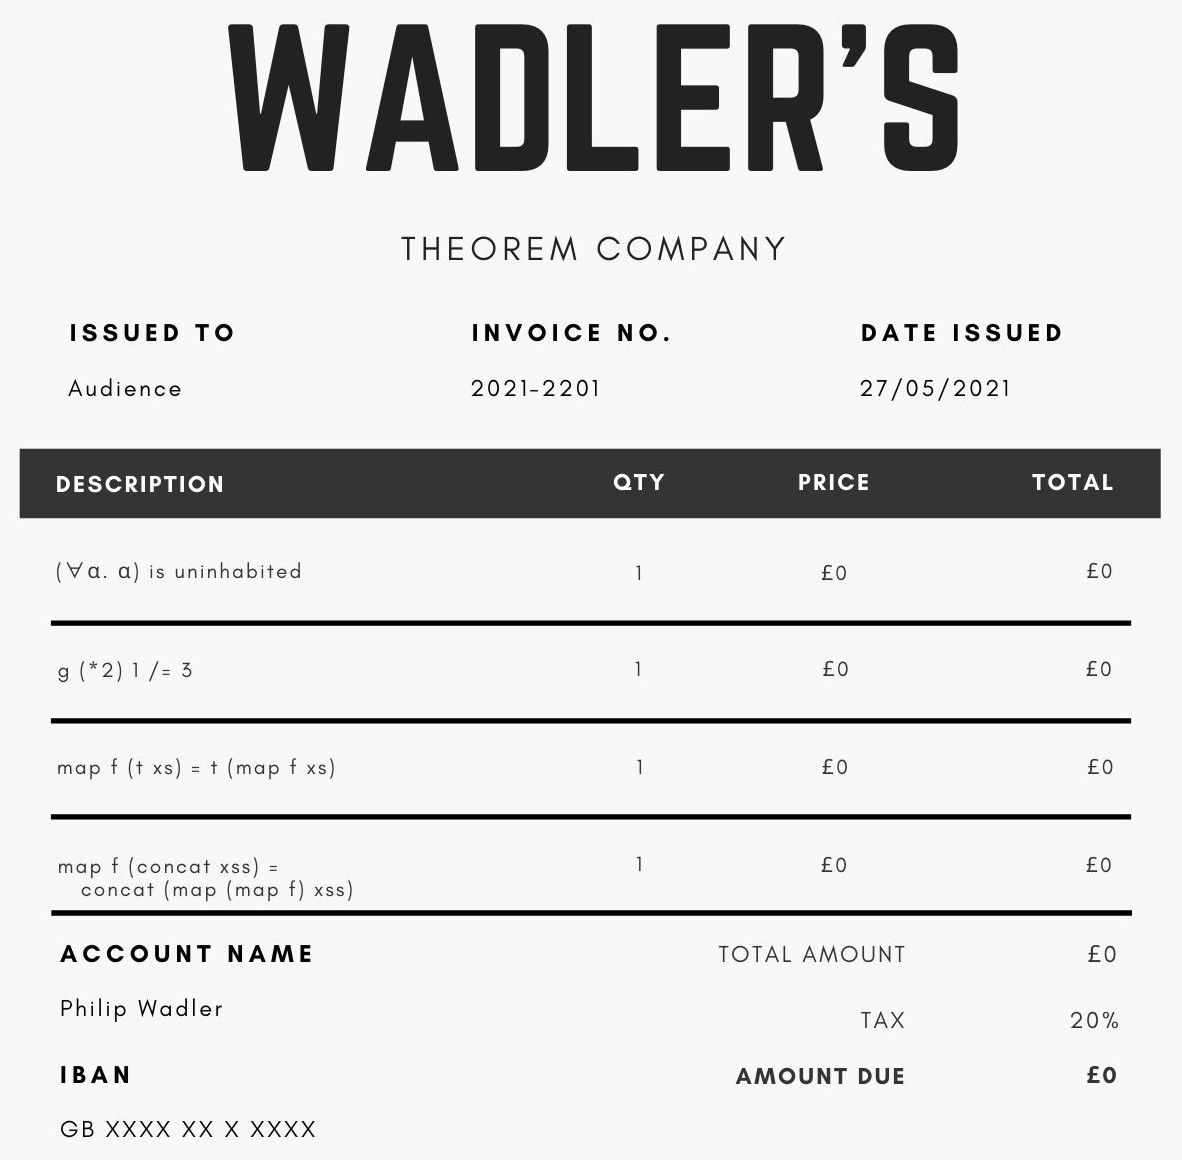
\includegraphics[scale=0.49]{wadlers.jpg}
\end{frame}
%----------------------------------------------------------------------------------------
%\begin{frame}[allowframebreaks]{References}
  %\bibliography{../paper/sources.bib}
  %\bibliographystyle{abbrv}
%\end{frame}

% \begin{frame}[allowframebreaks]{Image Sources}
% \begin{itemize}
% \end{itemize}
% \end{frame}

\begin{frame}{Natural Numbers}
Assume we have a base type $\mathbb{N}$ with $\suc : \mathbb{N}\to\mathbb{N}$.

\pause
Assume we are given some value $t : \forall \alpha.\, (\alpha\to\alpha)\to\alpha\to\alpha$, a type $\tau$, and values $s : \tau\to\tau$ and $z : \tau$.
What is the result of $t\,[\tau]\,s\,z$?

\pause
Set $R\coloneqq \bigl\{(n,\nf{(s^n\, z)})\mid n\in\mathbb{N}\bigr\}$ and note that $(\suc, s)\in\vint{\alpha\to\alpha}_{[\alpha\mapsto(\mathbb{N},\tau,R)]}$:\\
\pause If $(v_1,v_2)\in\vint{\alpha}_{[\alpha\mapsto(\mathbb{N},\tau,R)]}$
then $(v_1,v_2)=\bigl(n,\nf{(s^n\, z)}\bigr)$ for some $n$.
Thus $(\suc\,v_1,s\,v_2)\eqnf\bigl(n+1,\nf{(s^{n+1}\, z)}\bigr)\in R$.

\pause
Hence, $\bigl(t\,[\mathbb{N}]\,\suc\, 0,t\,[\tau]\,s\,z\bigr)\in\tint{\alpha}_{[\alpha\mapsto(\mathbb{N},\tau,R)]}$ by the Parametricity Theorem.
\pause So there is $v' : \mathbb{N}$ and $v : \tau$ such that
$t\,[\mathbb{N}]\,\suc\, 0\to^*v'$ and $t\,[\tau]\,s\,z\to^*v$ and $(v',v)\in R$.
\pause Hence $v \eqnf s^n\, z$ where $n$ is determined by $t\,[\mathbb{N}]\,\suc\, 0\to^*v'\eqnf n$.
\end{frame}

\begin{frame}{Negative Results II}
We cannot define a polymorphic equality function $\eq : \forall \alpha.\, \alpha\to\alpha\to\bool$:

We would get $\eq\,[\tau]\,v_1\,v_2 \eqnf \eq\,[\tau']\,(f\,v_1)\,(f\,v_2)$ for any $f : \tau\to\tau',v_1 : \tau,v_2 : \tau$.
\end{frame}


\end{document}
